
% pgf settings: shrink the tick labels a bit
\pgfplotsset{every tick label/.append style={font=\scriptsize}}

\newcommand{\scatterplotsize}{8cm}
\newcommand{\scatterplotxlabelshift}{1.5ex}
\newcommand{\scatterplotylabelshift}{-3ex}




\section{Experiments}
\label{experiments}

We implemented our approach in Fast Downward
(FD) \cite{helmert:jair-06}. We evaluate it, in turn, on IPC
benchmarks modified for oversubscription planning, and on a selection
of IPC benchmarks extended with action-set properties.

In all experiments, the base planner called by our SysS and SysW
algorithms on each search node
employs \hff\ \cite{hoffmann:nebel:jair-01} for search guidance.
%
%% The base planner configurations, used to solve/prove unsolvability
%% of a meta search node, are greedy best first search with $\hff$ and
%% preferred operators ($hff$) and conjunction learning $\hc$ with
%% $\hff$ as its base heuristic. \rebecca{ask Marcel how it is
%% called} \rebecca{Modification of hC to find deadends with an cost
%% bound}
%
The experiments were run on a cluster of Intel E5-2660 machines
running at 2.20 GHz, with time (memory) cut-offs of 30 minutes (4
GB).



 
\subsection{Oversubscription Planning}

% The net-benefit benchmarks don't give us anything new (the ones we
% could use are adopted from IPC ben chmarks anyhow).
%
%% \joerg{Rebecca/Michael: check out the IPC net-benefit benchmarks. Reviewers may naturally expect us to experiment with those, given our strong focus on oversubscription planning (actually this question came up in the discussion with the NASA guys yesterday). In the net-bnefit benchmarks, goal facts have rewards which we don't need. The question is whether, stripping away these rewards and imposing a plan-cost bound, we would get benchmarks not already covered by bour IPC experiments anyway. If the answer is "no", we can just say so in the paper. If the answer is "yes", it would be good (though probably not absolitely necessary) to experiment with these domains as well. In any case, we should know what the answer is.}

To evaluate our analysis of goal dependencies as per
Section~\ref{goaldep}, we modified all optimal-planning STRIPS IPC
domains up to IPC'18. Following Domshlak and
Mirkis \shortcite{domshlak:mirkis:jair-15}, for each benchmark task we
ran an optimal planner (\astar
with \hlmcut\ \cite{helmert:domshlak:icaps-09}) to determine the
optimal plan cost $C$, then obtained OSP tasks by setting the cost
bound to $b = x * C$ where $x \in \{0.25, 0.5, 0.75\}$. Our benchmark
set consists of 46 domains, and contains those tasks solved by the
optimal planner, and where the number of goal facts is $< 32$.
%
%% ; the latter is an artifact of our current implementation that
%% could be overcome in principle, though computing all MUGS for that
%% many goals is presumably typically infeasible anyway.
%
We extended conjunction learning \cite{steinmetz:hoffmann:ai-17} to
deal with cost bounds, thus enabling nogood learning and transfer in
SysS and SysW.


\setlength{\tabcolsep}{2pt}
\renewcommand{\arraystretch}{0.8}
\begin{figure*}[h!]
	\tiny
	%\centering 	\scriptsize
	\begin{tabular}{l|rr|rr|rr|rr||rr|rr|rr|rr||rr|rr|rr|rr}
		& \multicolumn{8}{c}{0.25} & \multicolumn{8}{c}{0.5} & \multicolumn{8}{c}{0.75}\\
		& \multicolumn{2}{c}{C} & \multicolumn{2}{c}{Cnr} & \multicolumn{2}{c}{max} & & & \multicolumn{2}{c}{C} & \multicolumn{2}{c}{Cnr} & \multicolumn{2}{c}{max} & & &  \multicolumn{2}{c}{C} & \multicolumn{2}{c}{Cnr} & \multicolumn{2}{c}{max} & &\\\hline
		& c & t & c & t & c & t & nodes & mugs & c & t & c & t & c & t & nodes & mugs &  c & t & c & t & c & t & nodes & mugs\\\hline
		airport (28) & 0.79 & 0.0017 & 0.79 & 0.0066 & 0.86 & 18.3645 & 7 & 2.05 & 0.54 & 3.5596 & 0.54 & 3.5753 & 0.68 & 3.769 & 5 & 1.47 & 0.29 & 0.0078 & 0.29 & 0.0079 & 0.68 & 0.0035 & 3 & 1\\
		barman (4) & 1 & 0.0047 & 1 & 0.0144 & 1 & 0.0563 & 9 & 3 & 1 & 52.8352 & 1 & 43.8564 & 1 & 8.1814 & 8 & 3 & 0 & - & 0 & - & 1 & - & - & -\\
		blocks (28) & 1 & 0.0001 & 0.93 & 0.0007 & 0.96 & 0.0077 & 393 & 5.69 & 0.96 & 0.0006 & 0.93 & 0.004 & 0.75 & 0.56 & 140 & 6.05 & 0.89 & 0.0077 & 0.86 & 0.0159 & 0.61 & 1.447 & 52 & 6.06\\
		data-network (12) & 0 & - & 0 & - & 1 & - & - & - & 0 & - & 0 & - & 1 & - & - & - & 0 & - & 0 & - & 1 & - & - & -\\
		depot (7) & 1 & 0.0008 & 1 & 0.0043 & 1 & 0.1156 & 38 & 3.71 & 1 & 1.7631 & 1 & 0.7123 & 1 & 10.9838 & 36 & 6.71 & 0.43 & 6.5403 & 0.43 & 1.5582 & 0.57 & 5.8422 & 12 & 2.67\\
		driverlog (13) & 1 & 0.0002 & 1 & 0.0013 & 1 & 0.0432 & 556 & 6.38 & 0.92 & 0.0137 & 0.92 & 0.0374 & 0.77 & 0.3713 & 388 & 13.4 & 0.69 & 3.2144 & 0.69 & 1.9891 & 0.62 & 9.1767 & 191 & 7.88\\
		elevators (40) & 0 & - & 0 & - & 1 & - & - & - & 0 & - & 0 & - & 1 & - & - & - & 0 & - & 0 & - & 0.83 & - & - & -\\
		floortile (13) & 0 & - & 0 & - & 0.46 & - & - & - & 0 & - & 0 & - & 0.15 & - & - & - & 0 & - & 0 & - & 0.15 & - & - & -\\
		freecell (15) & 1 & 0.0003 & 1 & 0.0054 & 1 & 0.15 & 17 & 4 & 0.4 & 0.0085 & 0.47 & 0.0175 & 1 & 0.1357 & 16 & 5.2 & 0 & - & 0 & - & 0.93 & - & - & -\\
		ged (15) & 0 & - & 0 & - & 0.67 & - & - & - & 0 & - & 0 & - & 0.67 & - & - & - & 0 & - & 0 & - & 0.67 & - & - & -\\
		grid (2) & 1 & 0.0002 & 1 & 0.0034 & 1 & 0.0138 & 6 & 1.5 & 1 & 0.0122 & 1 & 0.0177 & 1 & 1.2066 & 6 & 1.5 & 0.5 & 0.0018 & 1 & 0.004 & 1 & 0.02 & 3 & 1\\
		gripper (7) & 0.71 & 0.0079 & 0.71 & 0.0069 & 0.71 & 0.0172 & 1087 & 77.4 & 0.57 & 1.0907 & 0.57 & 0.1444 & 0.57 & 0.0733 & 286 & 87 & 0.43 & 1.4578 & 0.43 & 0.8578 & 0.71 & 0.0336 & 43 & 12.67\\
		hiking (9) & 1 & 0.0019 & 1 & 0.0029 & 1 & 0.1407 & 4 & 1.44 & 0.67 & 0.4672 & 0.67 & 0.3678 & 1 & 3.9923 & 4 & 1.67 & 0.22 & 2.5099 & 0.22 & 1.1453 & 1 & 0.9072 & 4 & 1\\
		logistics (26) & 1 & 0.0007 & 1 & 0.0036 & 0.85 & 4.5539 & 110 & 4.05 & 0.77 & 0.1136 & 0.85 & 0.0671 & 0.58 & 5.1033 & 48 & 4.53 & 0.54 & 0.3488 & 0.58 & 0.1775 & 0.46 & 0.2939 & 22 & 2.17\\
		miconic (141) & 0.47 & 0.0016 & 0.46 & 0.0044 & 0.4 & 0.0477 & 438 & 27.89 & 0.29 & 0.3027 & 0.35 & 0.0338 & 0.32 & 0.1269 & 66 & 17.78 & 0.25 & 0.9975 & 0.28 & 0.1975 & 0.32 & 0.091 & 20 & 5.54\\
		mprime (22) & 1 & 0.0002 & 1 & 0.0036 & 1 & 0.0115 & 4 & 1.32 & 1 & 0.0011 & 1 & 0.0044 & 1 & 0.3336 & 4 & 1.23 & 1 & 0.0167 & 1 & 0.026 & 1 & 16.9777 & 4 & 1.18\\
		mystery (17) & 1 & 0.0003 & 1 & 0.0052 & 1 & 0.0199 & 4 & 1.41 & 1 & 0.0018 & 1 & 0.0062 & 1 & 1.6016 & 4 & 1.35 & 0.82 & 0.0049 & 0.82 & 0.0134 & 0.88 & 1.513 & 4 & 1.15\\
		nomystery (14) & 0.71 & 0.0003 & 0.71 & 3 & 1 & 0.0321 & 76 & 5.4 & 0 & - & 0.07 & - & 0.71 & - & - & - & 0 & - & 0 & - & 0.57 & - & - & -\\
		openstacks (47) & 0.15 & 0.0016 & 0.15 & 24 & 0.51 & 0.1372 & 316 & 6.43 & 0.11 & 0.0177 & 0.11 & 0.0372 & 0.47 & 0.0163 & 33 & 4.2 & 0.11 & - & 0 & - & 0.43 & - & - & -\\
		org-syn (7) & 1 & 0.0002 & 0.86 & 0.0179 & 0.86 & 0.0486 & 40 & 3.17 & 1 & 0.0011 & 0.86 & 0.0198 & 0.86 & 0.0504 & 40 & 3.17 & 1 & 0.0013 & 0.86 & 0.0208 & 0.86 & 0.054 & 40 & 3.17\\
		org-syn-s (10) & 0.8 & 0.0007 & 0.6 & 0.0152 & 0.6 & 5.9967 & 64 & 3.17 & 0.5 & 0.0004 & 0.5 & 0.0062 & 0.6 & 0.0374 & 70 & 3 & 0.2 & 0.0003 & 0.2 & 0.0072 & 0.6 & 0.0293 & 129 & 6\\
		parcprinter (24) & 0 & - & 0 & - & 0.42 & - & - & - & 0 & - & 0 & - & 0.42 & - & - & - & 0 & - & 0 & - & 0.42 & - & - & -\\
		parking (5) & 1 & - & 0 & - & 0 & - & - & - & 0.2 & - & 0 & - & 0 & - & - & - & 0 & - & 0 & - & 0 & - & - & -\\
		pathways-noneg (5) & 1 & 0.0002 & 1 & 0.0009 & 1 & 1.5975 & 20 & 3.2 & 0.4 & 0.0002 & 0.4 & 0.0002 & 0.8 & 0.0043 & 4 & 1.5 & 0.2 & 0.0001 & 0.2 & 0.0002 & 0.8 & 0.0022 & 3 & 1\\
		pegsol (2) & 0 & - & 0 & - & 0 & - &  &  & 0 & - & 0 & - & 0 & - & - & - & 0 & - & 0 & - & 0 & - & - & -\\
		pipesworld-nt (17) & 1 & 0.0006 & 1 & 4 & 1 & 0.0336 & 40 & 3.35 & 0.94 & 0.5306 & 0.94 & 0.3581 & 0.94 & 1.7601 & 26 & 5 & 0.82 & 10.0899 & 0.82 & 13.0619 & 0.94 & 41.5442 & 18 & 4.14\\
		pipesworld-t (12) & 0.92 & 0.0003 & 0.92 & 4 & 1 & 0.0809 & 34 & 3.45 & 0.92 & 0.2643 & 0.92 & 0.2918 & 0.92 & 11.8348 & 31 & 5 & 0.75 & 0.4525 & 0.75 & 0.6277 & 0.75 & 18.627 & 15 & 3.13\\
		psr-small (49) & 1 & 0.0002 & 0.98 & 0.0007 & 0.98 & 0.0006 & 615 & 3.44 & 1 & 0.0009 & 0.98 & 0.0035 & 0.98 & 0.004 & 475 & 2.52 & 0.96 & 0.0055 & 0.92 & 0.0135 & 0.96 & 0.0637 & 83 & 1.78\\
		rovers (8) & 1 & 0.0097 & 1 & 0.0031 & 1 & 0.0873 & 163 & 18 & 0.88 & 0.6903 & 0.88 & 0.0918 & 0.88 & 1.8094 & 34 & 11.43 & 0.5 & 0.0016 & 0.88 & 0.0018 & 0.75 & 0.0024 & 6 & 1.5\\
		satellite (7) & 1 & 0.0002 & 1 & 0.0027 & 1 & 0.3211 & 176 & 5.57 & 0.86 & 0.0417 & 1 & 0.0461 & 0.86 & 1.2065 & 114 & 18.67 & 0.71 & 0.2023 & 0.86 & 0.1006 & 0.57 & 0.1612 & 51 & 13.25\\
		scanalyzer (23) & 0.57 & 0.0001 & 0.39 & 0.0012 & 0.39 & 0.0103 & 2359 & 12.67 & 0.39 & 0.0476 & 0.39 & 0.0198 & 0.39 & 0.1573 & 1939 & 45.78 & 0.22 & 0.131 & 0.22 & 0.0369 & 0.39 & 0.1435 & 550 & 30.8\\
		snake (7) & 0.57 & 0.0008 & 0.14 & 0.0151 & 0.14 & 0.1996 & 245 & 4 & 0 & - & 0 & - & 0.14 & - & - & - & 0 & - & 0 & - & 0.14 & - & - & -\\
		sokoban (50) & 0 & - & 0 & - & 0.98 & - & - & - & 0 & - & 0 & - & 0.94 & - & - & - & 0 & - & 0 & - & 0.84 & - & - & -\\
		storage (15) & 1 & 0.0003 & 1 & 1 & 1 & 0.0025 & 13 & 3.6 & 1 & 0.2554 & 1 & 0.0665 & 1 & 0.1762 & 11 & 3.73 & 0.93 & 9.902 & 0.93 & 3.744 & 1 & 0.9675 & 7 & 1.93\\
		termes (6) & 1 & 0.0008 & 0.33 & 0.0469 & 1 & 36 & 2881 & 2.5 & 0.17 & - & 0 & - & 0.17 & - & - & - & 0 & - & 0 &  & 0 & - & - & -\\
		tetris (6) & 0.83 & 0.0003 & 0.33 & 0.0088 & 0.33 & 0.0147 & 257 & 6.5 & 0.5 & 0.0133 & 0.33 & 0.0297 & 0.33 & 0.0307 & 205 & 10 & 0.33 & 0.8305 & 0.33 & 0.5429 & 0.5 & 0.1313 & 106 & 5.5\\
		tidybot (23) & 1 & 0.0032 & 1 & 0.0536 & 1 & 1.4659 & 16 & 2.57 & 0.7 & 3.9946 & 0.7 & 3.3744 & 1 & 34.3564 & 16 & 3 & 0.43 & 7.1982 & 0.3 & 10.1166 & 0.3 & 14.7701 & 15 & 3.5\\
		tpp (7) & 1 & 0.0002 & 1 & 1 & 1 & 24 & 37 & 3.86 & 1 & 0.0328 & 1 & 0.0201 & 0.86 & 0.2812 & 21 & 6.17 & 0.71 & 0.0469 & 0.86 & 0.0242 & 0.86 & 0.014 & 9 & 2.8\\
		transport (23) & 1 & 0.0004 & 1 & 0.0015 & 1 & 0.0154 & 17 & 3.04 & 1 & 0.0649 & 1 & 0.1057 & 1 & 1.0104 & 16 & 3.17 & 0.96 & 6.7547 & 0.96 & 4.1551 & 1 & 14.8687 & 12 & 2.05\\
		trucks (10) & 0.2 & 0.0001 & 0.2 & 0.0003 & 1 & 0.0012 & 13 & 3.5 & 0 & - & 0 & - & 0.6 & - & - & - & 0 & - & 0 & - & 0.6 & - & - & -\\
		visitall (14) & 0.71 & 0.0001 & 0.57 & 0.0002 & 0.64 & 0.0004 & 10292 & 19.88 & 0.71 & 0.0002 & 0.5 & 0.0013 & 0.57 & 0.0046 & 6930 & 38 & 0.57 & 0.0034 & 0.5 & 0.0087 & 0.5 & 0.0338 & 4533 & 38.29\\
		woodworking (29) & 0.45 & 0.0001 & 0.17 & 0.0006 & 0.24 & 0.0016 & 2148 & 17.8 & 0.1 & 0.0012 & 0.1 & 0.0058 & 0.17 & 0.0134 & 1426 & 29 & 0.07 & 0.0097 & 0.1 & 0.0802 & 0.17 & 0.1136 & 1093 & 17\\
		zenotravel (13) & 1 & 0.0008 & 1 & 0.0073 & 0.92 & 0.2413 & 122 & 8 & 0.69 & 0.0011 & 0.77 & 0.0045 & 0.62 & 0.0424 & 38 & 3.75 & 0.69 & 0.4634 & 0.69 & 0.3243 & 0.62 & 1.6294 & 26 & 2.38\\\hline
		(862) & 0.62 & 0.0012 & 0.58 & 0.0077 & 0.76 & 0.9414 & 632 & 8.05 & 0.48 & 2.0666 & 0.49 & 1.6665 & 0.68 & 2.7886 & 392 & 11.97 & 0.39 & 1.7662 & 0.39 & 1.3409 & 0.62 & 4.4643 & 245 & 6.95\\
	\end{tabular}

 
	\centering % 3 * 5 coverage, 3 * goal size, 3 * 2 fraction search tree
\begin{tabular}{l|rrrr||rrrr|rrrr|rrrr||rrr|rrr||rr|rr|rr}
	& \multicolumn{4}{c||}{Reference Points}  & \multicolumn{12}{c||}{Coverage, $x=$} & \multicolumn{6}{c||}{\#MUGS, $x=$} & \multicolumn{6}{c}{Search Tree Fraction, $x=$} \\
	   & \hlmcut & \multicolumn{3}{c||}{$\hc$} & \multicolumn{4}{c|}{0.25} & \multicolumn{4}{c|}{0.5} & \multicolumn{4}{c||}{0.75} & 0.25 & 0.5 & 0.75 & 0.25 & 0.5 & 0.75 & \multicolumn{2}{c|}{0.25} & \multicolumn{2}{c|}{0.5} & \multicolumn{2}{c}{0.75} \\\hline
					   & & \multicolumn{3}{c||}{$x=$} & \multicolumn{2}{c}{SysS} & \multicolumn{2}{c|}{SysW}& \multicolumn{2}{c}{SysS} & \multicolumn{2}{c|}{SysW}& \multicolumn{2}{c}{SysS} & \multicolumn{2}{c||}{SysW} 
	& & & & & & &\multicolumn{2}{c|}{Sys} & \multicolumn{2}{c|}{Sys} & \multicolumn{2}{c}{Sys}  \\
	domain  & - & 0.25 & 0.5 & 0.75 &  & $\hc$ &  & $\hc$ &  & $\hc$  &  & $\hc$ &  & $\hc$ &  & $\hc$ & \multicolumn{3}{c|}{avg} & \multicolumn{3}{c|}{max} & S & W & S & W & S & W \\\hline
	agricola (20) &	0 & - &- & -& - & - & - & - & - & - & - & - & -
			   & - & - & - & - & - & - & - & - & - & - & - & - & - & - & - \\
	airport (50) &	28 & 28 & 24 & 17  
		& 25 & 26 & 24 & \textbf{27}  & 19 & \textbf{21}  & 19 & \textbf{21}  & \textbf{19}  & 16 & \textbf{19}  & 16
	   & 2.7 & 2.0 & 1.2 & 11 & 5 & 4 & \textbf{0.67} & 0.76 & 0.88 & \textbf{0.71} & 1.00 & \textbf{0.61}\\
	barman (34) &	4 & 4 & 4 & 4 
		& 4 & 4 & 4 & 4 & 4 & 4 & 4 & 4 & \textbf{4}  & 0 & \textbf{4}  & \textbf{4} 
		   & 3.0 & 3.0 & 1.0 & 3 & 3 & 1 & \textbf{0.50} & 0.88 & 0.88 & 0.88 & - & - \\
	blocks (35) &	28 & 28 & 28 & 28
				& \textbf{28}  & \textbf{28}  & 27 & \textbf{28}  & 23 & \textbf{27}  & 21 & \textbf{27}  & 18 & 24 & 17 & \textbf{26}
				  & 7.6 & 10.8 & 14.1 & 39 & 30 & 57 & \textbf{0.19} & 0.97 & \textbf{0.39} & 0.93 & 0.78 & \textbf{0.72}\\
	childsnack (20) &	0 & - & - & -
		   & - & - & - & - & - & - & - & - & - & - & - & -
		 & - & - & - & - & - & - & - & - & - & - & - & - \\
	data-network (20) &	12 & 12 & 12 & 12
			& 12 & 12 & 12 & 12 & 12 & 12 & 12 & 12 & 11 & \textbf{12}  & 11 & \textbf{12}
			 & 1.7 & 1.5 & 1.2 & 3 & 3 & 2 &0.83 & \textbf{0.65} & 0.88 & \textbf{0.65} & 0.92 & \textbf{0.61}\\
	depot (22) &	7 & 7 & 7 & 6 
			& 7 & 7 & 7 & 7 & 7 & 7 & 7 & 7 & \textbf{4}  & 3 & \textbf{4}  & 3
			 & 4.0 & 7.0 & 4.5 & 6 & 12 & 10 & \textbf{0.34} & 0.94 & \textbf{0.52} & 0.91 & 0.89 & \textbf{0.68}\\ 
	driverlog (18) &	13 & 13 & 13 & 11 
		  & 13 & 13 & 13 & 13 & 10 & 11 & 10 & \textbf{12}  & 8 & \textbf{10} & 7 & \textbf{10}
			  & 7.0 & 18.2 & 8.7 & 22 & 45 & 17 & \textbf{0.19} & 0.98 & \textbf{0.58} & 0.86 & 0.85 & \textbf{0.50}\\
	elevators (50) &	40 & 40 & 40 & 35 
					& 40 & 40 & 40 & 40 & \textbf{40}  & 37 & 38 & 37 & \textbf{35}  & 26 & 31 & 26
				   & 3.9 & 4.9 & 3.2 & 8 & 13 & 8 & \textbf{0.37} & 0.94 & \textbf{0.67} & 0.89 & 0.92 & \textbf{0.71}\\
	floortile (36) &	13 & 13 & 13 & 6
					& 7 & 7 & 6 & \textbf{8}  & 2 & 2 & 2 & 2 & \textbf{2}  & 1 & \textbf{2}  & \textbf{2} 
				   & 175.6 & 66.0 & 31.5 & 697 & 71 & 33 & \textbf{0.12} & 0.99 & \textbf{0.67} & 0.80 & 0.97 & \textbf{0.28}\\
	freecell (80) &	15 & 15 & 15 & 13 
					& 15 & 15 & 15 & 15 & 15 & 15 & 15 & 15 & \textbf{14}  & 13 & 13 & 13
				  & 4.0 & 4.7 & 3.4 & 4 & 6 & 5 & \textbf{0.31} & 0.94 & \textbf{0.60} & 0.94 & 0.88 & \textbf{0.76}\\
	ged (20) &	15 & 15 & 15 & 11 
			& 15 & 15 & 15 & 15 & \textbf{15}  & 10 & 10 & 10 & 10 & \textbf{7}  & 10 & \textbf{7}
			 & 9.2 & 38.7 & 12.5 & 18 & 101 & 38 & \textbf{0.23} & 0.90 & \textbf{0.47} & 0.80 & \textbf{0.58} & 0.70\\
	grid (5) &	2 & 2 & 2 & 2 
			& 2 & 2 & 2 & 2 & 2 & 2 & 2 & 2 & 2 & 2 & 2 & 2
			 & 1.5 & 1.5 & 1.0 & 2 & 2 & 1 & 0.81  & \textbf{0.69} & 0.81 & \textbf{0.69} & 1.00 & \textbf{0.56} \\
	gripper (14) &	7 & 7 & 7 & 5 
					& \textbf{7}  & 5 & 5 & 5 & 4 & 4 & 4 & 4 & \textbf{4}  & 3 & \textbf{4}  & 3
				 & 458.3 & 87.0 & 39.5 & 1820 & 252 & 120 & \textbf{0.21} & 0.98 & \textbf{0.65} & 0.88 & 0.96 & \textbf{0.46}\\
	hiking (20) &	9 & 9 & 9 & 9 
				& 9 & 9 & 9 & 9 & 9 & 9 & 9 & 9 & 9 & 9 & 9 & 9
				& 1.4 & 1.4 & 1.0 & 2 & 2 & 1 & 0.89 & \textbf{0.61} & 0.89 & \textbf{0.61} & 1.00 & \textbf{0.61}\\
	logistics (60) &	26 & 26 & 26 & 20  
					& 24 & \textbf{26}  & 21 & \textbf{26}  & 15 & 19 & 14 & \textbf{20}  & 12 & 13 & 12 & \textbf{15}
				   & 6.3 & 6.0 & 2.9 & 25 & 22 & 7 & \textbf{0.31} & 0.95 & \textbf{0.68} & 0.84 & 0.90 & \textbf{0.63} \\
	miconic (150) &	141 & 120 & 76 & 50
					& \textbf{66}  & \textbf{66}  & 55 & 64 & \textbf{45}  & 40 & 44 & 43 & \textbf{41}  & 36 & 40 & 36
				  & 76.0 & 24.1 & 8.4 & 363 & 98 & 36 & \textbf{0.33} & 0.91 & \textbf{0.73} & 0.82 & 0.95 & \textbf{0.61}\\
	movie (30) &	30 & 30 & 30 & 30
				& 30 & 30 & 30 & 30 & 30 & 30 & 30 & 30 & 30 & 30 & 30 & 30
			   & 7.0 & 35.0 & 21.0 & 7 & 35 & 21 & \textbf{0.06} & 0.99 & \textbf{0.50} & 0.94 & 0.94 & \textbf{0.50}\\
	mprime (35) &	22 & 22 & 22 & 22
				& 22 & 22 & 22 & 22 & 22 & 22 & 22 & 22 & 22 & 22 & 22 & 22
				& 1.3 & 1.2 & 1.2 & 2 & 2 & 2 & 0.90 & \textbf{0.59} & 0.92 & \textbf{0.59} & 0.93 & \textbf{0.59}\\
	mystery (30) &	17 & 17 & 17 & 17 
				& 17 & 17 & 17 & 17 & 17 & 17 & 17 & 17 & 15 & \textbf{17}  & 15 & \textbf{17}
				 & 1.4 & 1.4 & 1.2 & 2 & 2 & 2 & 0.88 & \textbf{0.63} & 0.88 & \textbf{0.63} & 0.92 & \textbf{0.63}\\
	nomystery (20) &	14 & 14 & 14 & 13 
					& 14 & 14 & 14 & 14 & 10 & \textbf{12}  & 10 & \textbf{12}  & 8 & 8 & 8 & 8
				   & 7.3 & 18.5 & 5.8 & 18 & 47 & 13 & \textbf{0.20} & 0.96 & \textbf{0.63} & 0.92 & 0.87 & \textbf{0.61}\\
	openstacks (77) &	47 & 45 & 45 & 43
					& \textbf{45}  & \textbf{45}  & 37 & 43 & \textbf{45}  & 43 & 29 & 41 & \textbf{42}  & \textbf{42}  & 22 & 33
					& 15.3 & 14.2 & 12.3 & 25 & 25 & 23 & \textbf{0.06} & 0.99 & \textbf{0.05} & 0.99 & \textbf{0.18} & 0.97\\
	org-syn (20) &	7 & 7 & 7 & 7 
					& 7 & 7 & 7 & 7 & 7 & 7 & 7 & 7 & 7 & 7 & 7 & 7
				 & 5.1 & 5.1 & 5.1 & 12 & 12 & 12 & \textbf{0.23} & 0.94 & \textbf{0.23} & 0.94 & \textbf{0.23} & 0.94\\
	org-syn-s (13) &	10 & 10 & 10 & 9
					& \textbf{8}  & \textbf{8}  & 7 & \textbf{8}  & \textbf{8}  & \textbf{8}  & 7 & \textbf{8}  & \textbf{7}  & 6 & 6 & 6
				   & 5.2 & 7.2 & 8.3 & 12 & 28 & 36 & \textbf{0.20} & 0.95 & \textbf{0.23} & 0.95 & \textbf{0.32} & 0.89 \\
	parcprinter (26) &	24 & 20 & 20 & 20
					& 10 & 10 & 10 & \textbf{14}  & 10 & 10 & 10 & \textbf{14}  & 10 & 10 & 10 & \textbf{12}
					 & 3.8 & 8.2 & 5.0 & 14 & 24 & 10 & \textbf{0.44} & 0.98 & \textbf{0.61} & 0.95 & \textbf{0.72} & 0.85\\
	parking (40) &	5 & 5 & 5 & 1 
				& \textbf{5}  & \textbf{5}  & 4 & \textbf{5}  & 0 & \textbf{1}  & 0 & \textbf{1}  & 0 & 0 & 0 & 0
				 & 36.8 & 31.0 & - & 79 & 31 & - & 0.02 & 0.99 & - & - & - & - \\
	pathways (23) &	5 & 5 & 5 & 5 
					& 5 & 5 & 5 & 5 & 4 & \textbf{5}  & 4 & \textbf{5}  & 4 & 4 & 4 & 4
				  & 3.2 & 3.8 & 1.8 & 6 & 10 & 3 &\textbf{0.53} & 0.81 & 0.77 & 0.77 & 0.91 & \textbf{0.70}\\
	pegsol (2) &	2 & 2 & 2 & 2 
				& 0 & 0 & \textbf{2}  & \textbf{2}  & 0 & 0 & \textbf{2}  & \textbf{2}  & 0 & 0 & \textbf{2}  & \textbf{2}
			   & 7.0 & 23.5 & 64.0 & 8 & 41 & 122 & - & - & - & - & - & - \\
	pipesworld-nt (50) &	17 & 17 & 17 & 17 
						& 17 & 17 & 17 & 17 & \textbf{17}  & \textbf{17}  & 16 & \textbf{17}  & \textbf{16}  & 14 & \textbf{16}  & 14
					   & 3.7 & 6.4 & 3.8 & 8 & 31 & 17 & \textbf{0.44} & 0.89 & \textbf{0.73} & 0.84 & 0.88 & \textbf{0.66}\\
	pipesworld-t (50) &	12 & 12 & 12 & 11 
					& 12 & 12 & 12 & 12 & 11 & 11 & 11 & 11 & \textbf{9}  & 11 & \textbf{9}  & 10
					  & 3.6 & 5.0 & 3.7 & 7 & 15 & 12 & \textbf{0.43} & 0.94 & \textbf{0.67} & 0.87 & 0.90 & \textbf{0.63}\\
	psr-small (50) &	49 & 49 & 49 & 49 
					& 48 & 48 & \textbf{49}  & \textbf{49}  & 47 & 47 & 48 & \textbf{49}  & 46 & 46 & \textbf{48}  & \textbf{48}
					& 3.7 & 2.7 & 2.0  & 20 & 13 & 9 & 0.76 & \textbf{0.63} & 0.94 & \textbf{0.55} & 0.97 & \textbf{0.47}\\
	rovers (31) &	8 & 8 & 8 & 7 
				& 8 & 8 & 8 & 8 & 7 & 7 & 7 & 7 & \textbf{6}  & 5 & \textbf{6}  & 4
				& 18.0 & 11.4 & 3.8 & 95 & 35 & 12 & \textbf{0.36} & 0.93 & \textbf{0.74} & 0.84 & 0.91 & \textbf{0.59}\\
	satellite (19) &	7 & 7 & 7 & 6 
					& 7 & 7 & 7 & 7 & 6 & 6 & 6 & \textbf{7}  & 4 & 5 & 4 & \textbf{6}
				   & 5.6 & 26.9 & 14.7 & 7 & 76 & 36 & \textbf{0.19} & 0.97 & \textbf{0.49} & 0.94 & 0.88 & \textbf{0.73}\\
	scanalyzer (40) &	23 & 21 & 21 & 13 
						& \textbf{9}  & 15 & \textbf{9}  & 13 & 9 & 9 & 9 & 9 & \textbf{9}  & 5 & \textbf{9}  & \textbf{9}
					& 20.9 & 36.7 & 31.2 & 46 & 103 & 43 & \textbf{0.25} & 0.99 & \textbf{0.53} & 0.86 & \textbf{0.75} & 0.83\\
	snake (17) &	7 & 7 & 7 & 4 
				& 6 & 6 & 6 & 6 & 3 & 3 & 3 & 3 & \textbf{3}  & 1 & 2 & 1
			   & 10.5 & 21.0  & 44.3 & 16 & 27 & 77 & \textbf{0.13} & 0.92 & \textbf{0.32} & 0.86 & \textbf{0.58} & 0.73\\
	sokoban (50) &	50 & 50 & 49 & 41
					& \textbf{50}  & \textbf{50}  & 49 & \textbf{50}  & \textbf{46}  & 43 & 45 & 43 & \textbf{40}  & 30 & \textbf{40}  & 28
				 & 6.6 & 4.1 & 1.8 & 56 & 36 & 10 & \textbf{0.60} & 0.85 & 0.86 & \textbf{0.71} & 0.95 & \textbf{0.51}\\
	storage (30) &	15 & 15 & 15 & 15
				& 15 & 15 & 15 & 15 & 15 & 15 & 15 & 15 & \textbf{15}  & 14 & \textbf{15}  & 14
				 & 3.6 & 3.7 & 2.1 & 10 & 10 & 5 & \textbf{0.62} & 0.81 & 0.85 & \textbf{0.75} & 0.98 & \textbf{0.57}\\
	termes (20) &	6 & 6 & 4 & 1 
				& \textbf{6}  & \textbf{6}  & 5 & \textbf{6}  & \textbf{5}  & 1 & 1 & 2 & \textbf{1}  & 0 & 0 & 0
				 & 3.2 & 2.6 & 3.0 & 8 & 6 & 3 & \textbf{0.37} & 0.72 & 0.53 & 0.53  & - & - \\
	tetris (17) &	6 & 6 & 6 & 5 
				& \textbf{6}  & \textbf{6}  & 5 & \textbf{6}  & \textbf{4}  & 3 & 3 & 3 & \textbf{3}  & 2 & \textbf{3}  & 2
				& 29.7 & 32.8 & 7.3 & 81 & 82 & 11 & \textbf{0.26} & 0.98 & 0.81 & \textbf{0.77} & 0.97 & \textbf{0.41}\\
	tidybot (40) &	23 & 23 & 23 & 19
			   & 23 & 23 & 23 & 23 & \textbf{23}  & 22 & \textbf{23}  & 22 & 13 & 13 & 7 & \textbf{14}
				 & 3.1 & 3.3 & 3.4 & 4 & 6 & 6 & \textbf{0.38} & 0.92 & \textbf{0.41} & 0.92 & \textbf{0.75} & 0.84\\
	tpp (30) &	7 & 7 & 7 & 6 
			& 7 & 7 & 7 & 7 & 6 & \textbf{7}  & 6 & 6 & \textbf{6}  & 5 & \textbf{6}  & 5
			 & 4.1 & 8.9 & 4.2 & 9 & 25 & 11 & \textbf{0.43} & 0.86 & \textbf{0.67} & 0.83 & 0.96 & \textbf{0.66}\\
	transport (70) & 23 & 23 & 23  & 22
					& 23 & 23 & 23 & 23 & 23 & 23 & 23 & 23 & \textbf{23}  & 22 & 22 & 22
				   & 3.5 & 3.7 & 2.1 & 5 & 10 & 6 & \textbf{0.43} & 0.91 & \textbf{0.59} & 0.88 & 0.73 & \textbf{0.69}\\
	trucks (30) &	10 & 10 & 10 & 8 
			  & \textbf{10} & \textbf{10} & 9  & \textbf{10} & 6 & \textbf{7}  & 6 & \textbf{7}  & \textbf{5}  & 3 & \textbf{5}  & 4
				& 15.7 & 17.1 & 5.0 & 36 & 31 & 8 & \textbf{0.23} & 0.97 & \textbf{0.70} & 0.89 & 0.93 & \textbf{0.65}\\
	visitall (14) &	14 & 13 & 13 & 13 
					 & \textbf{13}  & \textbf{13}  & 10 & 10 & 9  & \textbf{10} & 8 & \textbf{10} & 6 & 6 & 7 & \textbf{8}
				  & 97.4 & 111.6 & 46.5 & 307 & 380 & 150 & \textbf{0.20} & 0.93 & \textbf{0.41} & 0.90 & 0.79 & \textbf{0.75}\\
	woodworking (35) &	29 & 25 & 25 & 25 
					& \textbf{23}  & \textbf{23}  & 12 & 15 & \textbf{9}  & \textbf{9}  & 5 & \textbf{9}  & 5 & 5 & 5 & 5
					 & 267.3 & 95.0 & 16.8 & 1030 & 192 & 26 & \textbf{0.02} & 0.99 & \textbf{0.27} & 0.93 & 0.72 & \textbf{0.52}\\
	zenotravel (20) &	13 & 13 & 12 & 9 
					& \textbf{13}  & \textbf{13}  & 12 & \textbf{13}  & \textbf{9}  & \textbf{9}  & 8 & \textbf{9}  & 8 & \textbf{9}  & 8 & \textbf{9}
					& 10.4 & 4.0 & 2.6 & 36 & 6 & 4 & \textbf{0.36} & 0.94 & \textbf{0.67} & 0.89 & 0.87 & \textbf{0.66}\\\hline
	Sum (1583)  & 862 & 828 & 776 & 670
		  & 733 & \textbf{740}  & 688 & 732 & 630 & 624 & 592 & \textbf{636}  & \textbf{556}  & 517 & 523 & 528 & &&&&&&&&&&

%31.1 & 18.7 & 10.7 & 113.4 & 45.6 & 24.0 & \textbf{0.38} & 0.90 & \textbf{0.63} & 0.82 & 0.83 & \textbf{0.65}\\
\end{tabular}
 
        \vspace{-0.2cm}
	\caption{Results on IPC benchmarks modified for oversubscription planning. Reference Points: related classical planning tasks (see text). Coverage: of our MUGS algorithms SysS and SysW, with vs.\ without conjunction learning \hc. \#MUGS: average/maximum number of MUGS, indicating explanation size (see text). Search Tree Fraction: fraction of worst-case search tree explored. Best performance in each part shown in \textbf{boldface}. Cost bounds set to $x$ times optimal cost.}
	\label{table:coverage_ipc}
        \vspace{-0.5cm}
\end{figure*}

Figure~\ref{table:coverage_ipc} shows our data. Consider first the
coverage data (leftmost two parts). To have some sort of measure of
how computationally difficult our proposed analysis is, we use
reference points from classical planning. First, the \hlmcut\ column
gives coverage for \astar\ with \hlmcut\ run on the original IPC
instance without a cost bound. This provides a comparison to solvable
optimal planning. Second, the \hc\ columns give coverage for search,
with nogood learning, on the respective cost-bounded instances, when
all goals must be achieved and thus the task is unsolvable. This
provides a comparison to proving unsolvability, in the same situation
where our approach computes all MUGS.
%
It is expected that our algorithms, solving a more complex problem,
will perform worse than the reference points.\footnote{Indeed, the
first reference point is an upper bound to our coverage, as only
solved instances are included in our benchmark set; and the second
reference point is an upper bound for SysW as it constitutes the first
search node in that algorithm.} The question is, \emph{how much
worse?}

As a short summary of the answer provided by
Figure~\ref{table:coverage_ipc} to that question, compared to
the \hlmcut\ reference point, taking the per-domain best of our four
algorithm configurations, for $x=0.25$ we get equal coverage in 36 of
the 46 domains, and in that sense are ``not much worse'' than optimal
planning. For larger cost bounds, the solvable goal subsets become
larger, and accordingly our analysis becomes harder. For $x=0.5$ we
get equal coverage in 23 domains, for $x=0.75$ in 13. The comparison
to the \hc\ proving-unsolvability reference points is qualitatively
similar, with equal coverage in 38, 25, and 20 domains for $x=0.25,
0.5, 0.75$ respectively. Overall, it seems fair to say that our
analyses can be feasible in many cases, in the sense of not being more
infeasible than the most closely related classical planning problems.

While comparing our algorithm configurations against each other is not
our focus here, observe in the rightmost part of
Figure~\ref{table:coverage_ipc} that both SysS and SysW suffer from
larger cost bounds, but that is less so for SysW. This is because, for
small cost bounds, solvable goal sets are small and thus SysS
terminates earlier; while for large cost bounds, solvable goal sets
are large and thus SysW terminates earlier. Conjunction learning (\hc\
in the table) is moderately beneficial.
%
%% Comparing SysS and SysW, with cost bound 0.25 both show better
%% coverage in 4 domains. Among those domains, in \woodworking\
%% and \openstacks\ SysS explores a much smaller fraction of the
%% meta-search tree than SysW (0.02 vs. 0.99 and 0.06 vs. 0.99). With
%% a cost bound of 0.5 SysW has better coverage in more domains (8
%% vs. 6). With cost 0.75 both show better coverage in 7
%% domains. Although SysW explores the smaller fraction of the
%% meta-search tree, SysS still demonstrates better coverage
%% overall. \rebecca{In this setting, finding a plan is easier than
%% proving unsolvability?}
%
%% The table shows that $\hc$ is useful with SysW, but for SysS only
%% with cost bound is $0.25$.

Consider finally the \#MUGS part of
Figure~\ref{table:coverage_ipc}. Observe that, if the user asks a
question ``Why $r$ rather than $p$?'', the answer are the properties
entailed by $p$, represented here through the smallest conjunctions
excluded by $p$. The number of such conjunctions is at most the number
of MUGS. So \#MUGS corresponds to worst-case answer/explanation
size. As the data shows, that size is often small, of a scale that
seems feasible for human inspection. 
%
%% (Taking the maximum rather than average per domain, the average across
%% domains is 113.4, 45.6, 24.0 for $x=0.25, 0.5, 0.75$ respectively.)
%% \rebecca{discus new mugs max columns}

%
%% The average MUGS size for a cost bound of 0.25 is small (1.32). It
%% is often the case that for these problems, you cannot reach any of
%% the goal facts. In that case, the MUGS will be the goals.







%%%%%%%%%%%%%%%%%%%%%%%%%%%%%%%%%%%%%%%%%%%%%%%%%%%%%%%%%%%%%%%%%%%%
%%%%%%%%%%%%%%%%%%%%%%%%%%%%%%%%%%%%%%%%%%%%%%%%%%%%%%%%%%%%%%%%%%%%
%%%%%%%%%%%%%%%%%%%%%%%%%%%%%%%%%%%%%%%%%%%%%%%%%%%%%%%%%%%%%%%%%%%%
%%%% SUBMISSION VERSION

\ifdefined\longflagdefined

\else

\subsection{Action-Set Properties}

To evaluate the use of our framework with more complex plan
properties, beyond goal facts, we experimented with the compilation of
action-set properties as per Section~\ref{compilation}. We selected
four IPC domains for extension with action-set properties, namely
NoMystery, Rovers, and TPP as considered in resource-constrained
planning \cite{nakhost:etal:icaps-12}, where minimum resource
requirements are known as per available problem generators; plus the
Blocksworld as an intuitively rather differently structured domain. In
all four domains, we use discrete resource consumption encoded into
the STRIPS model, enabling the use of trap
learning \cite{steinmetz:hoffmann:ijcai-17} which turns out to be
highly beneficial here.

In Blocksworld, we include two gripper hands and the action-set
properties ask whether a given gripper is used to pick up a given
block, or to stack a given pair of blocks. In NoMystery, the
properties are as in our illustrative example
(Section~\ref{illustrative-example}). In Rovers, the properties ask
whether a given rover or camera is used for a given observation. In
TPP, they ask whether given road segments are used, and whether given
goods are bought at given markets. In all cases, we vary the number of
action-set properties between 1 and 10. We fix the original goal facts
as hard goals, and we set the available resources to $x \in \{1.0,1.5,
2.0\}$ times the minimum needed to allow for costlier plans satisfying
some of the properties.

We created benchmark tasks with size parameters around the borderline
of feasibility. As reference points, we ran \astar\ with \hlmcut\
respectively trap learning on tasks where all (original goal facts
plus) action-set properties are hard goals.

For lack of space, we only summarize our data.\footnote{For IJCAI'19
review, full plots are at
{\scriptsize \url{https://www.dropbox.com/sh/boq29booqajj7ab/AACbKpiR6jdbeEzCldrvLfk4a?dl=0}}}
%
%% \footnote{The complete data is available in supplementary material
%% at the following anonymized link \joerg{insert URL here}.}
%
In Blocksworld and TPP, our techniques are moderately competitive with
the reference points. In NoMystery, they are vastly inferior. In
Rovers, they vastly surpass \hlmcut, matching the coverage of the
trap-learning reference point. Overall, it seems fair to say that our
analysis here is not exceedingly infeasible compared to related
classical planning problems.




\fi

%%%% END SUBMISSION VERSION
%%%%%%%%%%%%%%%%%%%%%%%%%%%%%%%%%%%%%%%%%%%%%%%%%%%%%%%%%%%%%%%%%%%%
%%%%%%%%%%%%%%%%%%%%%%%%%%%%%%%%%%%%%%%%%%%%%%%%%%%%%%%%%%%%%%%%%%%%
%%%%%%%%%%%%%%%%%%%%%%%%%%%%%%%%%%%%%%%%%%%%%%%%%%%%%%%%%%%%%%%%%%%%







%%%%%%%%%%%%%%%%%%%%%%%%%%%%%%%%%%%%%%%%%%%%%%%%%%%%%%%%%%%%%%%%%%%%
%%%%%%%%%%%%%%%%%%%%%%%%%%%%%%%%%%%%%%%%%%%%%%%%%%%%%%%%%%%%%%%%%%%%
%%%%%%%%%%%%%%%%%%%%%%%%%%%%%%%%%%%%%%%%%%%%%%%%%%%%%%%%%%%%%%%%%%%%
%%%% PRE-FINAL AND SUPPLEMENTARY MATERIAL VERSION

\ifdefined\longflagdefined

\subsection{Action-Set Properties}

\begin{figure*}[htb]
\centering\centering
%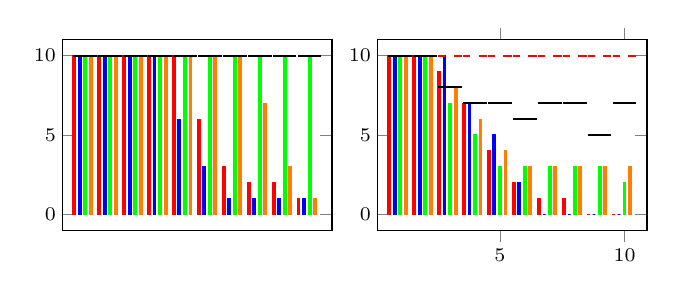
\begin{tikzpicture}
\tiny
    \begin{axis}[
    width =5cm,
    height=4cm,
    enlarge x limits = 0.1,
    enlarge y limits = 0.1,
    legend columns=1,
    ybar,
    bar width=1pt,
    ymin = 0,
    ymax = 10,
	compat=1.6,
	%title=c 100,
	%ylabel=goals 05,
	xticklabels={,,},
	xtick style={draw=none},
	at={(0,0)},
]
\addplot+[ybar, bar shift =-4.0pt, red,
]
plot coordinates {
(04, 10) %c_100
(05, 10) %c_100
(06, 6) %c_100
(01, 10) %c_100
(02, 10) %c_100
(08, 2) %c_100
(07, 3) %c_100
(03, 10) %c_100
(09, 2) %c_100
(10, 1) %c_100
};
\label{plot:props_bu_hff_94}
\addplot+[ybar, bar shift =-2.0pt, blue,
]
plot coordinates {
(04, 10) %c_100
(05, 6) %c_100
(06, 3) %c_100
(01, 10) %c_100
(02, 10) %c_100
(08, 1) %c_100
(07, 1) %c_100
(03, 10) %c_100
(09, 1) %c_100
(10, 1) %c_100
};
\label{plot:props_td_hff_94}
\addplot+[ybar, bar shift =0.0pt, green,
]
plot coordinates {
(04, 10) %c_100
(05, 10) %c_100
(06, 10) %c_100
(01, 10) %c_100
(02, 10) %c_100
(08, 10) %c_100
(10, 10) %c_100
(03, 10) %c_100
(09, 10) %c_100
(07, 10) %c_100
};
\label{plot:props_bu_trap_94}
\addplot+[ybar, bar shift =2.0pt, orange,
]
plot coordinates {
(04, 10) %c_100
(05, 10) %c_100
(06, 10) %c_100
(01, 10) %c_100
(02, 10) %c_100
(08, 7) %c_100
(07, 10) %c_100
(03, 10) %c_100
(09, 3) %c_100
(10, 1) %c_100
};
\label{plot:props_td_trap_94}

%lmcut
\addplot+[only marks, mark = -, mark options = {thick, red, dashed}, mark size = 0.15cm, black,
]
plot coordinates {
(01, 10)
(02, 10)
(03, 10)
(04, 10)
(05, 10)
(06, 10)
(07, 10)
(08, 10)
(09, 10)
(10, 10)
};

%trap first meta node top down
\addplot+[only marks, mark = -, mark options = {thick, black}, mark size = 0.15cm, black,
]
plot coordinates {
(01, 10)
(02, 10)
(03, 10)
(04, 10)
(05, 10)
(06, 10)
(07, 10)
(08, 10)
(09, 10)
(10, 10)
};

    \end{axis}
    \hfill
    
%\node[draw, align=center] (test) at (8,-18) {
%\ref{plot:props_bu_hff_94} props-bu-hff\\
%\ref{plot:props_td_hff_94} props-td-hff\\
%\ref{plot:props_bu_trap_94} props-bu-trap\\
%\ref{plot:props_td_trap_94} props-td-trap\\
%};

    \begin{axis}[
    width = 5cm,
    height=4cm,
    enlarge x limits = 0.1,
    enlarge y limits = 0.1,
    legend columns=1,
    ybar,
    bar width=1pt,
    ymin = 0,
    ymax = 10,
compat=1.6,
%title=c 150,
%ylabel=goals 6,
at={(4cm,0)},
]
\addplot+[ybar, bar shift =-4.0pt, red,
]
plot coordinates {
(08, 1) %c_150
(09, 0) %c_150
(03, 9) %c_150
(06, 2) %c_150
(07, 1) %c_150
(10, 0) %c_150
(04, 7) %c_150
(05, 4) %c_150
(01, 10) %c_150
(02, 10) %c_150
};
\label{plot:props_bu_hff_75}
\addplot+[ybar, bar shift =-2.0pt, blue,
]
plot coordinates {
(08, 0) %c_150
(09, 0) %c_150
(03, 10) %c_150
(06, 2) %c_150
(07, 0) %c_150
(10, 0) %c_150
(04, 7) %c_150
(05, 5) %c_150
(01, 10) %c_150
(02, 10) %c_150
};
\label{plot:props_td_hff_75}
\addplot+[ybar, bar shift =0.0pt, green,
]
plot coordinates {
(08, 3) %c_150
(09, 3) %c_150
(03, 7) %c_150
(06, 3) %c_150
(07, 3) %c_150
(10, 2) %c_150
(04, 5) %c_150
(05, 3) %c_150
(01, 10) %c_150
(02, 10) %c_150
};
\label{plot:props_bu_trap_75}
\addplot+[ybar, bar shift =2.0pt, orange,
]
plot coordinates {
(08, 3) %c_150
(09, 3) %c_150
(10, 3) %c_150
(06, 3) %c_150
(07, 3) %c_150
(03, 8) %c_150
(04, 6) %c_150
(05, 4) %c_150
(01, 10) %c_150
(02, 10) %c_150
};
\label{plot:props_td_trap_75}

%lmcut
\addplot+[only marks, mark = -, mark options = {thick, red, dashed}, mark size = 0.15cm, black,
]
plot coordinates {
(02, 10)
(01, 10)
(04, 10)
(03, 10)
(07, 10)
(08, 10)
(06, 10)
(10, 10)
(05, 10)
(09, 10)
};

%trap first meta node top down
\addplot+[only marks, mark = -, mark options = {thick, black}, mark size = 0.15cm, black,
]
plot coordinates {
(01, 10)
(02, 10)
(03, 8)
(04, 7)
(05, 7)
(06, 6)
(07, 7)
(08, 7)
(09, 5)
(10, 7)
};
    \end{axis}
    \hfill
    
%\node[draw, align=center] (test) at (8,-18) {
%\ref{plot:props_bu_hff_75} props-bu-hff\\
%\ref{plot:props_td_hff_75} props-td-hff\\
%\ref{plot:props_bu_trap_75} props-bu-trap\\
%\ref{plot:props_td_trap_75} props-td-trap\\
%%};



\end{tikzpicture}

\includegraphics{data/action_set_properties/barchart/barchart.pdf}
\vspace{-0.6cm}
\caption{Coverage results on IPC benchmarks extended with action-set properties.}
\label{fig:barcharts}
\vspace{-0.2cm}
\end{figure*}

To evaluate the use of our framework with more complex plan
properties, beyond goal facts, we experimented with the compilation of
action-set properties as per Section~\ref{compilation}. We selected
four IPC domains for extension with action-set properties, namely
NoMystery, Rovers, and TPP as considered in resource-constrained
planning \cite{nakhost:etal:icaps-12}, where minimum resource
requirements are known as per available problem generators; plus the
Blocksworld as an intuitively rather differently structured domain. In
all four domains, we use discrete resource consumption encoded into
the STRIPS model, enabling the use of trap
learning \cite{steinmetz:hoffmann:ijcai-17} which turns out to be
highly beneficial here.

In Blocksworld, we include two gripper hands and the action-set
properties ask whether a given gripper is used to pick up a given
block, or to stack a given pair of blocks. In NoMystery, the
properties are as in our illustrative example
(Section~\ref{illustrative-example}). In Rovers, the properties ask
whether a given rover or camera is used for a given observation. In
TPP, they ask whether given road segments are used, and whether given
goods are bought at given markets. In all cases, we vary the number of
action-set properties between 1 and 10. We fix the original goal facts
as hard goals, and we set the available resources to $x \in \{1.0,1.5,
2.0\}$ times the minimum needed to allow for costlier plans satisfying
some of the properties.

We created benchmark tasks with size parameters around the borderline
of computational feasibility for our analyses, given our time/memory
limits. In Blocksworld, we used 5 -- 8 blocks; in NoMystery, our tasks
have 2 trucks, 6 locations, and 4 -- 7 packages; in Rovers, they have
2 rovers, 5 waypoints, and 4 -- 7 science objectives; in TPP, we use 5
markets, 1 depot, and 4 -- 7 goods. In all domains, we vary the number
of goal facts (and associated objects) between 4 and 7. We create 10
base instances for each size-parameter setting, which are then
modified for our experiments with different initial resource levels,
and action-set properties to be considered.
%
%% \begin{enumerate}
%% \item The resource constrained \textit{rovers} domain. Problems were generated with 2 rovers, 5 waypoints. Action properties are to use a specific rover for a sample or an observation, or to use a specific camera for an observation. 
%% \item The \textit{blocksworld} domain with 2 grippers, modified such that picking up or unstacking a block costs high or low energy depending upon which gripper is used. Problems were generated scaling from 3 to 10 blocks. Action properties are to use a specific gripper to pick up a specific block, or to use any gripper to stack a specific pair of blocks at any point in the plan.
%% \item The resource constrained \textit{TPP} domain. Problems were generated with 5 markets and 1 depot. Properties are to use or not use particular road segments, and preferred markets for goods.
%% \item The resource constrained \textit{nomystery} domain, described in the example. Problems were generated with 6 locations and 2 trucks.
%% \end{enumerate}

To have some comparison measure for performance, again we use
classical-planning reference points, based on \astar\ with \hlmcut,
and on search with trap learning, respectively. We now run these
reference points on tasks where all (original goal facts plus)
action-set properties are hard goals. These tasks may be solvable (in
which case \astar\ with \hlmcut\ tends to be better) or unsolvable (in
which case trap learning tends to be better). The configurations of
our own algorithm are SysS and SysW as before, now with vs.\ without
trap learning (and transfer).

Figure~\ref{fig:barcharts} shows the coverage
data. \ifdefined\suppflagdefined To give an overview, we show \else
For space reasons, we show only \fi one row per domain, fixing the
number of hard goals at the feasibility borderline. Smaller numbers of
goal facts tend to be quite easy, larger ones mostly infeasible, with
variance depending on the domain and
algorithm. \ifdefined\suppflagdefined
Appendix~\ref{data-action-set-properties} gives complete data for each
of the four domains. 
%\else Complete data for each of the four domains
%is available in an online TR at \joerg{insert TR-URL here}. \fi

In Blocksworld, the best of our techniques are moderately competitive
with the \hlmcut\ reference point (which starts to lose coverage when
one more block is added). They match the performance of the other
reference point for $x=1.0$, and surpass it for larger $x$ where trap
learning incurs a prohibitive overhead. NoMystery is the most
problematic domain in terms of performance, with all our techniques
lagging far behind the two reference points. In Rovers,
though, \astar\ with \hlmcut\ is much less effective than our
techniques, which match the full coverage of the trap-learning
reference point. TPP is similar to Blocksworld in that our techniques
are moderately competitive with the reference points. 
%\joerg{statement where coverage for these starts to go down} 
Trap learning is highly
beneficial in all cases except Blocksworld with $x>1.0$. Overall, it
seems fair to say that our action-set property dependency analysis is
not exceedingly infeasible compared to related classical planning
problems.


\fi

%%%% END PRE-FINAL AND SUPPLEMENTARY MATERIAL VERSION
%%%%%%%%%%%%%%%%%%%%%%%%%%%%%%%%%%%%%%%%%%%%%%%%%%%%%%%%%%%%%%%%%%%%
%%%%%%%%%%%%%%%%%%%%%%%%%%%%%%%%%%%%%%%%%%%%%%%%%%%%%%%%%%%%%%%%%%%%
%%%%%%%%%%%%%%%%%%%%%%%%%%%%%%%%%%%%%%%%%%%%%%%%%%%%%%%%%%%%%%%%%%%%



































%%%%%%%%%%%%%%%%%%%%%%%%%%%%%%%%%%%%%%%%%%%%%%%%%%%%%%%%%%%%%%%%%%%%
%%%%%%%%%%%%%%%%%%%%%%%%%%%%%%%%%%%%%%%%%%%%%%%%%%%%%%%%%%%%%%%%%%%%
%%%%%%%%%%%%%%%%%%%%%%%%%%%%%%%%%%%%%%%%%%%%%%%%%%%%%%%%%%%%%%%%%%%%
%%% FIRST SHORT VERSION

%% \subsubsection*{Action-Set Properties}

%% \begin{figure*}[htb]
%% \centering\centering
%% %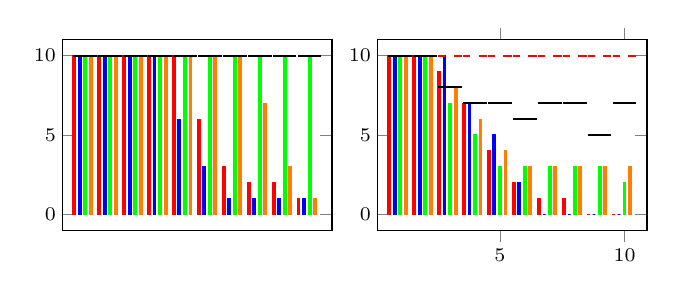
\begin{tikzpicture}
\tiny
    \begin{axis}[
    width =5cm,
    height=4cm,
    enlarge x limits = 0.1,
    enlarge y limits = 0.1,
    legend columns=1,
    ybar,
    bar width=1pt,
    ymin = 0,
    ymax = 10,
	compat=1.6,
	%title=c 100,
	%ylabel=goals 05,
	xticklabels={,,},
	xtick style={draw=none},
	at={(0,0)},
]
\addplot+[ybar, bar shift =-4.0pt, red,
]
plot coordinates {
(04, 10) %c_100
(05, 10) %c_100
(06, 6) %c_100
(01, 10) %c_100
(02, 10) %c_100
(08, 2) %c_100
(07, 3) %c_100
(03, 10) %c_100
(09, 2) %c_100
(10, 1) %c_100
};
\label{plot:props_bu_hff_94}
\addplot+[ybar, bar shift =-2.0pt, blue,
]
plot coordinates {
(04, 10) %c_100
(05, 6) %c_100
(06, 3) %c_100
(01, 10) %c_100
(02, 10) %c_100
(08, 1) %c_100
(07, 1) %c_100
(03, 10) %c_100
(09, 1) %c_100
(10, 1) %c_100
};
\label{plot:props_td_hff_94}
\addplot+[ybar, bar shift =0.0pt, green,
]
plot coordinates {
(04, 10) %c_100
(05, 10) %c_100
(06, 10) %c_100
(01, 10) %c_100
(02, 10) %c_100
(08, 10) %c_100
(10, 10) %c_100
(03, 10) %c_100
(09, 10) %c_100
(07, 10) %c_100
};
\label{plot:props_bu_trap_94}
\addplot+[ybar, bar shift =2.0pt, orange,
]
plot coordinates {
(04, 10) %c_100
(05, 10) %c_100
(06, 10) %c_100
(01, 10) %c_100
(02, 10) %c_100
(08, 7) %c_100
(07, 10) %c_100
(03, 10) %c_100
(09, 3) %c_100
(10, 1) %c_100
};
\label{plot:props_td_trap_94}

%lmcut
\addplot+[only marks, mark = -, mark options = {thick, red, dashed}, mark size = 0.15cm, black,
]
plot coordinates {
(01, 10)
(02, 10)
(03, 10)
(04, 10)
(05, 10)
(06, 10)
(07, 10)
(08, 10)
(09, 10)
(10, 10)
};

%trap first meta node top down
\addplot+[only marks, mark = -, mark options = {thick, black}, mark size = 0.15cm, black,
]
plot coordinates {
(01, 10)
(02, 10)
(03, 10)
(04, 10)
(05, 10)
(06, 10)
(07, 10)
(08, 10)
(09, 10)
(10, 10)
};

    \end{axis}
    \hfill
    
%\node[draw, align=center] (test) at (8,-18) {
%\ref{plot:props_bu_hff_94} props-bu-hff\\
%\ref{plot:props_td_hff_94} props-td-hff\\
%\ref{plot:props_bu_trap_94} props-bu-trap\\
%\ref{plot:props_td_trap_94} props-td-trap\\
%};

    \begin{axis}[
    width = 5cm,
    height=4cm,
    enlarge x limits = 0.1,
    enlarge y limits = 0.1,
    legend columns=1,
    ybar,
    bar width=1pt,
    ymin = 0,
    ymax = 10,
compat=1.6,
%title=c 150,
%ylabel=goals 6,
at={(4cm,0)},
]
\addplot+[ybar, bar shift =-4.0pt, red,
]
plot coordinates {
(08, 1) %c_150
(09, 0) %c_150
(03, 9) %c_150
(06, 2) %c_150
(07, 1) %c_150
(10, 0) %c_150
(04, 7) %c_150
(05, 4) %c_150
(01, 10) %c_150
(02, 10) %c_150
};
\label{plot:props_bu_hff_75}
\addplot+[ybar, bar shift =-2.0pt, blue,
]
plot coordinates {
(08, 0) %c_150
(09, 0) %c_150
(03, 10) %c_150
(06, 2) %c_150
(07, 0) %c_150
(10, 0) %c_150
(04, 7) %c_150
(05, 5) %c_150
(01, 10) %c_150
(02, 10) %c_150
};
\label{plot:props_td_hff_75}
\addplot+[ybar, bar shift =0.0pt, green,
]
plot coordinates {
(08, 3) %c_150
(09, 3) %c_150
(03, 7) %c_150
(06, 3) %c_150
(07, 3) %c_150
(10, 2) %c_150
(04, 5) %c_150
(05, 3) %c_150
(01, 10) %c_150
(02, 10) %c_150
};
\label{plot:props_bu_trap_75}
\addplot+[ybar, bar shift =2.0pt, orange,
]
plot coordinates {
(08, 3) %c_150
(09, 3) %c_150
(10, 3) %c_150
(06, 3) %c_150
(07, 3) %c_150
(03, 8) %c_150
(04, 6) %c_150
(05, 4) %c_150
(01, 10) %c_150
(02, 10) %c_150
};
\label{plot:props_td_trap_75}

%lmcut
\addplot+[only marks, mark = -, mark options = {thick, red, dashed}, mark size = 0.15cm, black,
]
plot coordinates {
(02, 10)
(01, 10)
(04, 10)
(03, 10)
(07, 10)
(08, 10)
(06, 10)
(10, 10)
(05, 10)
(09, 10)
};

%trap first meta node top down
\addplot+[only marks, mark = -, mark options = {thick, black}, mark size = 0.15cm, black,
]
plot coordinates {
(01, 10)
(02, 10)
(03, 8)
(04, 7)
(05, 7)
(06, 6)
(07, 7)
(08, 7)
(09, 5)
(10, 7)
};
    \end{axis}
    \hfill
    
%\node[draw, align=center] (test) at (8,-18) {
%\ref{plot:props_bu_hff_75} props-bu-hff\\
%\ref{plot:props_td_hff_75} props-td-hff\\
%\ref{plot:props_bu_trap_75} props-bu-trap\\
%\ref{plot:props_td_trap_75} props-td-trap\\
%%};



\end{tikzpicture}

%% \includegraphics{data/action_set_properties/barchart/barchart.pdf}
%% \vspace{-0.6cm}
%% \caption{Coverage results on IPC benchmarks extended with action-set properties.}
%% \label{fig:barcharts}
%% \vspace{-0.2cm}
%% \end{figure*}

%% To evaluate the use of our framework with more complex plan
%% properties, beyond goal facts, we experimented with the compilation of
%% action-set properties as per Section~\ref{compilation}. We selected
%% four IPC domains for extension with action-set properties, namely
%% NoMystery, Rovers, and TPP as considered in resource-constrained
%% planning \cite{nakhost:etal:icaps-12}, where optimal resource
%% requirements are known as per available problem generators; plus the
%% Blocksworld as an intuitively rather differently structured domain. In
%% all four domains, we use discrete resource consumption encoded into
%% the STRIPS model, enabling the use of trap
%% learning \cite{steinmetz:hoffmann:ijcai-17} which turns out to be
%% highly beneficial here.

%% We set the available resources to $x \in \{1.0,1.5,
%% 2.0\}$ times the minimum needed, and we chose the size parameters in a
%% way targetting the borderline of computational feasibility given our
%% time/memory limits. We vary the number of hard goals between 4 and 7,
%% and the number of action-set properties between 1 and 10. In
%% NoMystery, the action-set properties are as in the illustrative
%% example given in Section~\ref{illustrative-example}. In Blocksworld,
%% we include two gripper hands and the action-set properties ask whether
%% a particular gripper is used to pick up a particular block, or to
%% stack a particular pair of blocks. In Rovers, the properties ask
%% whether a particular rover or camera is used for a particular
%% observation. In TPP, they ask whether particular road segments are
%% used, and whether particular goods are bought at particular markets.

%% %% \begin{enumerate}
%% %% \item The resource constrained \textit{rovers} domain. Problems were generated with 2 rovers, 5 waypoints. Action properties are to use a specific rover for a sample or an observation, or to use a specific camera for an observation. 
%% %% \item The \textit{blocksworld} domain with 2 grippers, modified such that picking up or unstacking a block costs high or low energy depending upon which gripper is used. Problems were generated scaling from 3 to 10 blocks. Action properties are to use a specific gripper to pick up a specific block, or to use any gripper to stack a specific pair of blocks at any point in the plan.
%% %% \item The resource constrained \textit{TPP} domain. Problems were generated with 5 markets and 1 depot. Properties are to use or not use particular road segments, and preferred markets for goods.
%% %% \item The resource constrained \textit{nomystery} domain, described in the example. Problems were generated with 6 locations and 2 trucks.
%% %% \end{enumerate}

%% Figure~\ref{fig:barcharts} shows coverage data, comparing against the
%% same reference points as before. For space reasons, we show only one
%% row per domain, fixing the number of hard goals at the feasibility
%% borderline (smaller numbers of hard goals tend to be quite easy,
%% larger ones largely infeasible, with variance depending on the domain
%% etc). Our algorithm configurations here are SysS and SysW as before,
%% now with vs.\ without trap learning (which can deal only with STRIPS,
%% not with the cost bounds used in oversubscription planning
%% above). Similarly as for Figure~\ref{table:coverage_ipc}, the data
%% shows that our analyses can be feasible compared to the reference
%% points; although that depends, of course, on the domain and on
%% instance size. Trap learning and transfer turns out to be extremely
%% useful here, vastly outperforming the non-learning algorithm in many
%% cases.
